\documentclass[12pt, a4paper, oneside]{article}\usepackage[]{graphicx}\usepackage[]{color}
%% maxwidth is the original width if it is less than linewidth
%% otherwise use linewidth (to make sure the graphics do not exceed the margin)
\makeatletter
\def\maxwidth{ %
  \ifdim\Gin@nat@width>\linewidth
    \linewidth
  \else
    \Gin@nat@width
  \fi
}
\makeatother

\definecolor{fgcolor}{rgb}{0.345, 0.345, 0.345}
\newcommand{\hlnum}[1]{\textcolor[rgb]{0.686,0.059,0.569}{#1}}%
\newcommand{\hlstr}[1]{\textcolor[rgb]{0.192,0.494,0.8}{#1}}%
\newcommand{\hlcom}[1]{\textcolor[rgb]{0.678,0.584,0.686}{\textit{#1}}}%
\newcommand{\hlopt}[1]{\textcolor[rgb]{0,0,0}{#1}}%
\newcommand{\hlstd}[1]{\textcolor[rgb]{0.345,0.345,0.345}{#1}}%
\newcommand{\hlkwa}[1]{\textcolor[rgb]{0.161,0.373,0.58}{\textbf{#1}}}%
\newcommand{\hlkwb}[1]{\textcolor[rgb]{0.69,0.353,0.396}{#1}}%
\newcommand{\hlkwc}[1]{\textcolor[rgb]{0.333,0.667,0.333}{#1}}%
\newcommand{\hlkwd}[1]{\textcolor[rgb]{0.737,0.353,0.396}{\textbf{#1}}}%

\usepackage{framed}
\makeatletter
\newenvironment{kframe}{%
 \def\at@end@of@kframe{}%
 \ifinner\ifhmode%
  \def\at@end@of@kframe{\end{minipage}}%
  \begin{minipage}{\columnwidth}%
 \fi\fi%
 \def\FrameCommand##1{\hskip\@totalleftmargin \hskip-\fboxsep
 \colorbox{shadecolor}{##1}\hskip-\fboxsep
     % There is no \\@totalrightmargin, so:
     \hskip-\linewidth \hskip-\@totalleftmargin \hskip\columnwidth}%
 \MakeFramed {\advance\hsize-\width
   \@totalleftmargin\z@ \linewidth\hsize
   \@setminipage}}%
 {\par\unskip\endMakeFramed%
 \at@end@of@kframe}
\makeatother

\definecolor{shadecolor}{rgb}{.97, .97, .97}
\definecolor{messagecolor}{rgb}{0, 0, 0}
\definecolor{warningcolor}{rgb}{1, 0, 1}
\definecolor{errorcolor}{rgb}{1, 0, 0}
\newenvironment{knitrout}{}{} % an empty environment to be redefined in TeX

\usepackage{alltt} % Paper size, default font size and one-sided paper
%\graphicspath{{./Figures/}} % Specifies the directory where pictures are stored
%\usepackage[dcucite]{harvard}
\usepackage{rotating}
\usepackage{amsmath}
\usepackage{setspace}
\usepackage{pdflscape}
\usepackage[flushleft]{threeparttable}
\usepackage{multirow}
\usepackage[comma, sort&compress]{natbib}% Use the natbib reference package - read up on this to edit the reference style; if you want text (e.g. Smith et al., 2012) for the in-text references (instead of numbers), remove 'numbers' 
\usepackage{graphicx}
%\bibliographystyle{plainnat}
\bibliographystyle{agsm}
\usepackage[colorlinks = true, citecolor = blue, linkcolor = blue]{hyperref}
%\hypersetup{urlcolor=blue, colorlinks=true} % Colors hyperlinks in blue - change to black if annoying
%\renewcommand[\harvardurl]{URL: \url}
 \usepackage{listings}
 \usepackage{color}
\definecolor{mygrey}{gray}{0.95}
\lstset{backgroundcolor=\color{mygrey}}
\IfFileExists{upquote.sty}{\usepackage{upquote}}{}
\begin{document}
\title{Analysis of level 4 BSc Finance and Investment results (2013-14)}
\author{Rob Hayward}
%\date{\today}
\maketitle
%\begin{abstract}
%erehrere
%\end{abstract}

\subsection*{Conclusions}
\begin{itemize}
\item Taking students through clearing does not appear to be a problem
\item Students arriving with lower level qualifications tend to have the greatest difficulties.  However, this is less pronounced in Financial Accouting and Professional skills.  Can we draw some \emph{good practice} from these modules?
\item Overseas have greater difficulties than average.  This reinforces the suggestion put forward by Tracey Taylor that these students require additional support. 
\end{itemize}

The total number of students was 34.  The outcomes recorded by the summer Exam Board are in Table \ref{tabref:out}.  

% latex table generated in R 3.0.2 by xtable 1.7-1 package
% Tue Jul 22 07:21:07 2014
\begin{table}[ht]
\centering
\begin{tabular}{rr}
  \hline
 & Number of Students \\ 
  \hline
FWD &   3 \\ 
  Pass &  19 \\ 
  Refer &   6 \\ 
  Withdrawal &   6 \\ 
   \hline
\end{tabular}
\caption{Outcome of Level 4 BSc. Finance and Investsment Students} 
\label{tabref:out}
\end{table}

The figures show that 8.82 percent of the students failed and were asked to withdraw;  55.88 percent passed at the first attempt; 17.65 were referred and 17.65 withdrew before taking exams.  

There are four issues to consider in detail: the first is the proportion of students who do not complete the first year; the second is the performance of students taken onto the course through clearing; the third is the relationship between student entry grades and the level four performance; the final issue is that of the performance of overseas students. 

\subsection*{Proportion of students completing level 4}
Though the University counts \emph{fail-withdraw} and \emph{withdraw} as the same, it is clear from an investigation of the student files that these are two distinct categories.  The second group includes switched to another course and those leaving the course for non-academic reasons. 

For example, Eleanor Alabaster withdrew for``family and personal reasons'';  Erikas Gringaliunas withdrew because for financial difficulties, he was an overseas student from Lithuania, had no financial support and found it too expensive in Brighton; Laura Battle withdrew because she found it impossible to keep up with the mathematical elements of Economics and had not settled in Brighton; Jack Bridges transferred out to Sport and Exercise Science; Craig O'Neill withdrew as a result of his poor health and his disability; Samuel Peka transferred to Computer Science. 

\subsection*{Performance of clearing students}
There were 6 students taken  onto the course through clearing.  It is evident from the box-plot in Figure \ref{boxplot1} and from Table \ref{tabref:out2} that these were relatively strong students.   

\begin{knitrout}
\definecolor{shadecolor}{rgb}{0.969, 0.969, 0.969}\color{fgcolor}\begin{figure}[h]

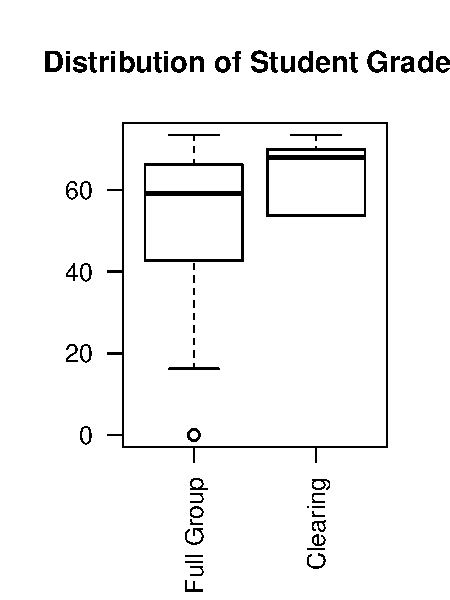
\includegraphics[width=\maxwidth]{figure/boxplot1} \caption[Comparison of total and clearing grades]{Comparison of total and clearing grades\label{fig:boxplot1}}
\end{figure}


\end{knitrout}
The box plot shows the distribution of grades; the solid black line is the median grade for all students and for clearing students respectively; the box gives the interquartile range (showing the range of half the students for each group); the whiskers extent to one-and-a-half times the interquartile range; zeros are outliers that are beyond the whiskers. 

% latex table generated in R 3.0.2 by xtable 1.7-1 package
% Tue Jul 22 07:21:07 2014
\begin{table}[ht]
\centering
\begin{tabular}{rr}
  \hline
 & Number of Students \\ 
  \hline
FWD &   0 \\ 
  Pass &   4 \\ 
  Refer &   2 \\ 
  Withdrawal &   0 \\ 
   \hline
\end{tabular}
\caption{Outcome of Level 4 BSc. Finance and Investsment Students joined throgh clearing} 
\label{tabref:out2}
\end{table}


\subsection*{Entry grades and performance}
\begin{knitrout}
\definecolor{shadecolor}{rgb}{0.969, 0.969, 0.969}\color{fgcolor}\begin{figure}[h]

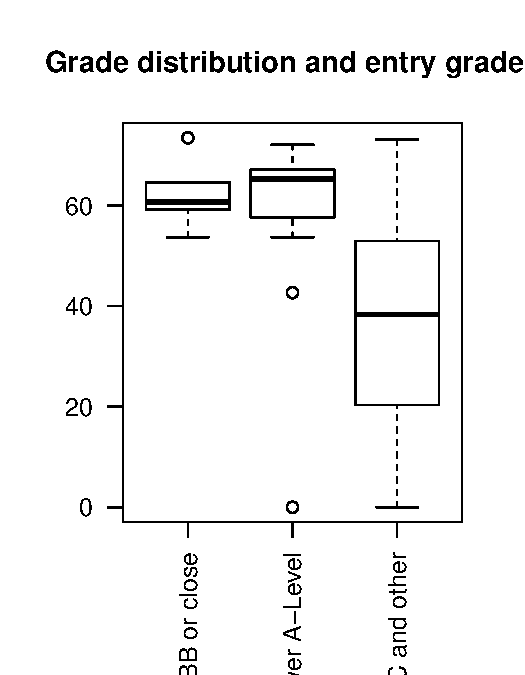
\includegraphics[width=\maxwidth]{figure/boxplot2} \caption[Entry grades and student performance]{Entry grades and student performance\label{fig:boxplot2}}
\end{figure}


\end{knitrout}

It is difficult to analyse the relationship between entry grades and student performance.  Students have been categorised into three levels of qualification:  A levels that are close to the ABB course entry requirement; Other A-levels with grades below AAB; and, non-A-level, primarily BETC qualifications.  The categorisation is a little imprecise.  However, unsurprisingly, there is a strong correlation between the entry grades and the end of year result.

It is possible to do some more detailed analysis of where the students with lower grades are falling down. They do particularly badly realtive to the overall average in EConomics EC161, Finance FN162 and Financial Skills FN142.   The difference between the students arriving with lower level qualifications and the average is less pronounced Financial Accounting FA183 and Personal and Academic Skills ML150. 
%<<reg, echo=FALSE, results='asis'>>=
%nicetable3 <- xtable(lm(da$Mark ~ da$Alevel -1), caption = "Level 4 grade %relative to A-level category", digits = 2)
%nicetable3
%@

\subsection*{The performance of overseas students}
\begin{knitrout}
\definecolor{shadecolor}{rgb}{0.969, 0.969, 0.969}\color{fgcolor}
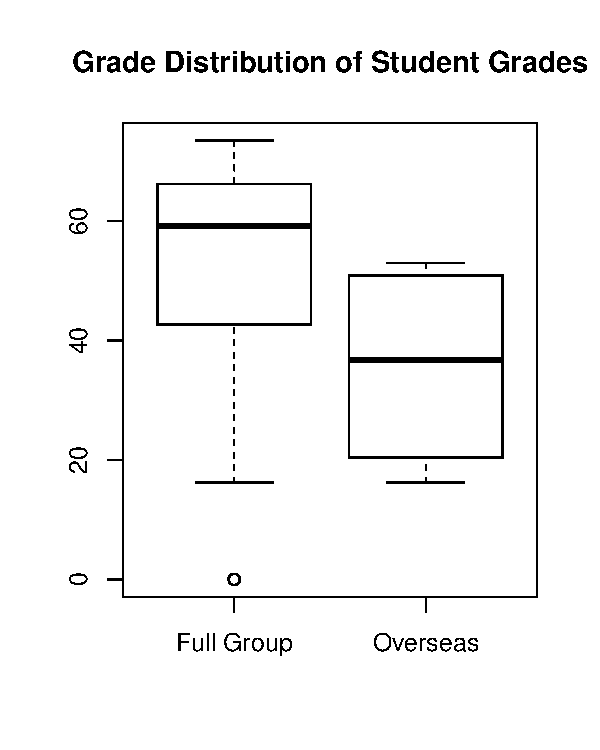
\includegraphics[width=\maxwidth]{figure/boxplot3} 

\end{knitrout}

Overseas students have to overcome cultural and language barriers in addition to the issues faced by other students.  The students are identified by their \emph{overseas} funding category.  The box-plot, constructed in the same way as outlined above, shows that the average overall level four mark for overseas students is 35.65 percent compared to 50.67 percent for the whole cohort.  


\end{document}
